\documentclass[a4paper, 12pt]{article}  % добавить leqno в [] для нумерации слева

%%% Работа с русским языком
\usepackage{cmap}
\usepackage[utf8]{inputenc}
\usepackage[english, russian]{babel}
\usepackage{pscyr}

%%% Дополнительная работа с математикой
\usepackage{amsmath,amsfonts,amssymb,amsthm,mathtools} % AMS
\usepackage{icomma} % "Умная" запятая

%% Номера формул
\mathtoolsset{showonlyrefs=true} % Показывать номера только у тех формул, на которые есть \eqref{} в тексте.

%% Шрифты
\usepackage{euscript} % Шрифт Евклид
\usepackage{mathrsfs} % Красивый матшрифт

%% Первый абзац после секшиона
\usepackage{indentfirst}

%% Свои команды
\DeclareMathOperator{\pphi}{\mathop{\varphi}}
\DeclareMathOperator{\eps}{\mathop{\varepsilon}}
\DeclareMathOperator{\conj}{\mathbb{\&}}

%% Перенос знаков в формулах (по Львовскому)
\newcommand*{\hm}[1]{#1\nobreak\discretionary{}
	{\hbox{$\mathsurround=0pt #1$}}{}}

%% Поля
\usepackage[left=1cm, right=1.4cm, top=1cm, bottom=1.3cm]{geometry}

%% Графика
\usepackage{tikz}

%% Переименовать список литературы
\addto\captionsrussian{\def\refname{Литература}}

%%% Заголовок
\author{Мат.клуб ``Тифаретник'' по С. Клини}
\title{Введение в метаматематику на троечку}
\date{\today}

%%% Эпиграф
\usepackage{epigraph}
\setlength\epigraphwidth{9cm}

%%% Работа с картинками
\usepackage{graphicx}  % Для вставки рисунков
\graphicspath{{images/}{images2/}}  % папки с картинками
\setlength\fboxsep{3pt} % Отступ рамки \fbox{} от рисунка
\setlength\fboxrule{1pt} % Толщина линий рамки \fbox{}
\usepackage{wrapfig} % Обтекание рисунков и таблиц текстом

%%% Добавляем код. Окружение lstlisting
\usepackage{listings}
\usepackage{color}
\definecolor{mygreen}{rgb}{0,0.6,0}
\definecolor{bggray}{RGB}{244,244,244}
\definecolor{mygray}{rgb}{0.5,0.5,0.5}
\definecolor{mymauve}{rgb}{0.58,0,0.82}
\lstset
{
	backgroundcolor=\color{bggray},   % choose the background color; you must add \usepackage{color} or \usepackage{xcolor}; should come as last argument
	basicstyle=\footnotesize,        % the size of the fonts that are used for the code
	breakatwhitespace=false,         % sets if automatic breaks should only happen at whitespace
	breaklines=true,                 % sets automatic line breaking
	captionpos=b,                    % sets the caption-position to bottom
	commentstyle=\color{mygreen},    % comment style
	deletekeywords={...},            % if you want to delete keywords from the given language
	escapeinside={\%*}{*)},          % if you want to add LaTeX within your code
	extendedchars=true,              % lets you use non-ASCII characters; for 8-bits encodings only, does not work with UTF-8
	%	firstnumber=1000,                % start line enumeration with line 1000
	%	frame=single,	                   % adds a frame around the code
	keepspaces=true,                 % keeps spaces in text, useful for keeping indentation of code (possibly needs columns=flexible)
	keywordstyle=\color{blue},       % keyword style
	language=c,                 	 % the language of the code
	morekeywords={*,...},            % if you want to add more keywords to the set
	numbers=none,                    % where to put the line-numbers; possible values are (none, left, right)
	numbersep=5pt,                   % how far the line-numbers are from the code
	numberstyle=\tiny\color{mygray}, % the style that is used for the line-numbers
	rulecolor=\color{black},         % if not set, the frame-color may be changed on line-breaks within not-black text (e.g. comments (green here))
	showspaces=false,                % show spaces everywhere adding particular underscores; it overrides 'showstringspaces'
	showstringspaces=false,          % underline spaces within strings only
	showtabs=false,                  % show tabs within strings adding particular underscores
	stepnumber=2,                    % the step between two line-numbers. If it's 1, each line will be numbered
	stringstyle=\color{mymauve},     % string literal style
	tabsize=3,	                     % sets default tabsize to 2 spaces
	title=\lstname                   % show the filename of files included with \lstinputlisting; also try caption instead of title	
}

%%% Ссылки
\usepackage{hyperref}

%%% Окружения
\theoremstyle{definition}
\newtheorem{theorem}{Теорема}
\newtheorem*{definition}{Определение}
\newtheorem*{pr}{Доказательство}

%%% Цифры в кружке
\newcommand*\circled[1]{\tikz[baseline=(char.base)]{
		\node[shape=circle,draw,inner sep=2pt] (char) {#1};}}

%%% Перечисление кастомное
\usepackage{enumitem}

%%% Естественный вывод
\usepackage{bussproofs}

%%% Несколько колонок для перечислений
\usepackage{multicol}

\usepackage{array}

\begin{document}
	\maketitle
	
	\epigraph{
		Формальные ограничители нужны человеку всегда,
			
		Они как огнетушители, а это, бля, не ерунда.
	}{Кровосток -- Снайпер}


	\begin{definition}[\textsection 16,  Формальные символы]
		\leavevmode	
		\begin{itemize}
			\setlength\itemsep{-3pt}
			\item \textit{Логические символы}: 
				$\supset$(влечёт), $\conj$(и), $\vee$(или),
				$\neg$(не), $\forall$(для всех), $\exists$(существует)
			\item \textit{Символы предикатов}: $=$(равняется)
			\item \textit{Символы функций}: 
				$+$(сложить с), $\cdot$(умножить на), $\backprime$(следующий за)
			\item \textit{Индивидуальные символы}: $0$(нуль)
			\item \textit{Переменные}: $a$, $b$, $c$, \dots
			\item \textit{Скобки}: $($, $)$
		\end{itemize}
	\end{definition}
	
	\begin{definition}[\textsection 17]
		\leavevmode			
		\begin{enumerate}
			\setlength\itemsep{-3pt}	
			\item $0$ есть \textit{терм}
			\item Каждая переменная есть \textit{терм}
			\item Если $s$ и $t$ --- \textit{термы}, то
			\begin{multicols}{4}
				\begin{enumerate}
				\item $(s)+(t)$          --- \textit{терм}
				\item $(s) \cdot (t)$    --- \textit{терм}
				\item $(s)^{\backprime}$ --- \textit{терм}
				\end{enumerate}
			\end{multicols}
			\item Никаких других \textit{термов}, кроме определённых согласно 1--3, нет.
		\end{enumerate}
	\end{definition}

	\begin{definition}[\textsection 17]
		\leavevmode				
		\begin{enumerate}
			\setlength\itemsep{-3pt}	
			\item Если $s$ и $t$ --- \textit{термы}, то $(s)=(t)$ --- \textit{формула}
			\item Если $A$ и $B$ --- \textit{формулы}, то
			\begin{multicols}{3}
				\begin{enumerate}
				\item $(A) \supset (B)$ --- \textit{формула}
				\item $(A) \conj\: (B)$ --- \textit{формула}
				\item $(A) \vee (B)$    --- \textit{формула}
				\item $\neg (A)$        --- \textit{формула}
				\end{enumerate}
			\end{multicols}
			\item Если $x$ --- переменная, а $A$ --- \textit{формула}, то 
			\begin{multicols}{3}
				\begin{enumerate}
				\item $\forall x (A)$ --- \textit{формула}
				\item $\exists x (A)$ --- \textit{формула}
				\end{enumerate}
			\end{multicols}
			\item Никаких других \textit{формул}, кроме определённых согласно 1--3, нет.
		\end{enumerate}
	\end{definition}
	
	\begin{definition}[\textsection 18]
		Вхождение $x$ в формулу $A$ называется \textit{связанным} (или вхождением в качестве 
		\textit{связанной переменной}), если оно является вхождением в квантор $\forall x$ или $\exists x$
		или в область действия квантора $\forall x$ или $\exists x$; в противном случае вхождение
		называется \textit{свободным}. 	
	\end{definition}

	\begin{definition}[\textsection 18]
		\textit{Подстановка терма $t$ вместо} переменной $x$ в терм или формулу $A$ состоит в одновременной
		 замене	каждого \textit{свободного вхождения} $x$ в $A$ на вхождение $t$.		
	\end{definition}

	\begin{definition}[\textsection 18]
		Будем говорить, что терм $t$ \textit{свободен при свободных вхождениях} переменной $x$ в 
		формулу $A(x)$, если никакое свободное вхождение $x$ в $A(x)$ не входит в область действия 
		какого-нибудь квантора $\forall y$ или $\exists y$, где $y$ --- переменная из $t$
		(т.е. входящая в $t$).  		
	\end{definition}

	\newpage
	
	{
		\centering
		\section*{Постулаты формальной системы (\textsection 19)}
	}
		\subsubsection*{Dramatis personae}
			В постулатах 1--8 $A, B$ и $C$ --- формулы. В 9--13 $x$ --- переменная, $A(x)$ --- формула, 
			$C$ --- формула, не содержащая свободно $x$, а $t$ --- терм, свободный для $x$ в $A(x)$.
		
		\subsection*{Группа А. Постулаты исчисления предикатов}
		
		\subsubsection*{Группа А1. Постулаты исчисления высказываний}
			\begin{multicols}{2}
				\begin{itemize}[label={}]
				\setlength\itemsep{0pt}	
				\item \circled{1a} $A \supset (B \supset A)$
				\item \circled{1b} $(A \supset B) \supset ((A \supset (B \supset C)) \supset (A \supset C))$
				\item \circled{4a} $A \conj B \supset A$
				\item \circled{4b} $A \conj B \supset B$
				\item \circled{5a} $A \supset A \vee B$
				\item \circled{5b} $B \supset A \vee B$
				\item \circled{2} 
					\AxiomC{$A, A \supset B $}
					\UnaryInfC{$B$}
					\DisplayProof
				\item \circled{3} $A \supset (B \supset A \conj B)$
				\item \circled{6} $(A \supset C) \supset ((B \supset C) \supset (A \vee B \supset C))$
				\item \circled{7} $(A \supset B) \supset ((A \supset \neg B) \supset \neg A)$
				\item \circled{$8^{\circ}$} $\neg \neg A \supset A$
				\item[\vspace{\fill}]
				\end{itemize}
			\end{multicols}
		
		\subsubsection*{Группа А2. (Дополнительные) Постулаты исчисления предикатов}
		\begin{multicols}{2}
			\begin{itemize}[label={}]
			\item \circled{9}
				\AxiomC{$C \supset A(x)$}
				\UnaryInfC{$C \supset \forall x A(x)$}
				\DisplayProof
			\item \circled{10} $\forall x A(x) \supset A(t)$
			\item \circled{11} $A(t) \supset \exists x A(x)$
			\item \circled{12} 
				\AxiomC{$A(x) \supset C$}
				\UnaryInfC{$\exists x A(x) \supset C$}
				\DisplayProof
			\end{itemize}
		\end{multicols}
		
		\subsection*{Группа B. (Дополнительные) Постулаты арифметики}
			\begin{multicols}{2}
				\begin{itemize}[label={}]
				\setlength\itemsep{0pt}	
				\item \circled{13} $A(0) \conj \forall x (A(x) \supset A(x^{\backprime})) \supset A(x)$
				\item \circled{14} $a^{\backprime} = b^{\backprime} \supset a = b$
				\item \circled{15} $\neg a^{\backprime} = 0$
				\item \circled{16} $a = b \supset (a = c \supset b = c)$
				\item \circled{17} $a = b \supset a^{\backprime} = b^{\backprime}$
				\item \circled{18} $a + 0 = a$
				\item \circled{19} $a + b^{\backprime} = (a + b)^{\backprime}$
				\item \circled{20} $a \cdot 0 = 0$
				\item \circled{21} $a \cdot b^{\backprime} = a \cdot b + a$
				\item[\vspace{\fill}]				
				\end{itemize}
			\end{multicols}
		
		\begin{definition}[\textsection 19]
			Формула является \textit{аксиомой}, если она имеет форму одну из \circled{1a}, 
			\circled{1b}, \circled{3}--\circled{8}, \circled{10}, \circled{11}, \circled{13} или она
			есть одна из \circled{14}--\circled{21}.  		
		\end{definition}
	
		\begin{definition}[\textsection 19]
			Формула является \textit{непосредственным следствием} (из) одной или двух других формул,
			если она имеет форму, указанную под чертой, тогда как другая (не) имеет(ют) форму(ы),
			указанную (не) над чертой в \circled{2}, \circled{9} или \circled{12}.    		
		\end{definition}
	
		\begin{definition}[\textsection 19]
			Постулаты \circled{2}, \circled{9} и \circled{12} мы называем 
			\textit{правилами вывода}. Для любого (фиксированного) выбора $A$ и $B$ или $x$, $A(x)$
			и $C$, подчинённого отмеченным выше условиям, формулы указанные над чертой, являются
			\textit{посылкой} (\textit{первой} и \textit{второй посылкой} соответственно), а 
			формула, указанная под чертой, является \textit{заключением} применения правила вывода.    		
		\end{definition}
		
	\subsection*{Формальный вывод}
	
	\begin{definition}[\textsection 20]
		Если дан перечень $D_1, \dots, D_l(l\ge0)$ формул, то непустая конечная последовательность формул
		называется \textit{формальным выводом из исходных формул} $D_1, \dots, D_l$, если каждая формула
		этой последовательности является или одной из формул $D_1, \dots, D_l$, или аксиомой, или
		непосредственным следствием из предыдущих формул последовательности. Вывод называется выводом
		\textit{своей последней} формулы $E$, и эта формула называется \textit{выводимой из} исходных
		формул (обозначается $D_1, \dots, D_l \vdash E$), а также \textit{заключением} (или 
		\textit{конечной формулой}) вывода.
	\end{definition}
	
	\begin{definition}[\textsection 20, Общие свойства $\vdash$]
		\leavevmode
		\begin{itemize}
			\setlength\itemsep{-3pt}
			\item $\Gamma \vdash E$, если $E$ входит в список $\Gamma$
			\item Если $\Gamma \vdash E$, то $\Delta, \Gamma \vdash E$ для любого перечня $\Delta$
				(Любая доказуемая выводима из любых исходных)
			\item Если $\Gamma \vdash E$, то $\Delta \vdash E$, где $\Delta$ получается из $\Gamma$
				путём перестановки формул $\Gamma$ или опускания любых таких формул, которые 
				тождественны с другими остающимися
			\item Если $\Gamma \vdash E$, то $\Delta \vdash E$, где $\Delta$ получается из $\Gamma$
				опусканием любых формул $\Gamma$, которые являются доказуемыми или выводимыми из
				остающихся формул $\Gamma$.
		\end{itemize}
	\end{definition}
	
	\begin{theorem}[\textsection 21, О дедукции]
		Для исчисления высказываний, если $\Gamma, A \vdash B$, то 
		$\Gamma \vdash A \supset B$.
	\end{theorem}

	\setcounter{theorem}{0}
	
	\begin{theorem}[\textsection 22, полная]
		 Для исчисления предикатов (или полной арифметической формальной системы), если 
		$\Gamma, A \vdash B$, причём все свободные переменные остаются фиксированными 
		для последней исходной формулы, то $\Gamma \vdash A \supset B$.
	\end{theorem}

	\begin{definition}[\textsection 23]
		Переменная ``$x$'' приписанная к символу ``$\vdash$'' в качестве верхнего индекса
		отличает применение правила \circled{9} или \circled{12} по отношению к $x$ 
		при построении результирующего вывода.		
	\end{definition}

	\begin{theorem}[\textsection 23]
		В следующих правилах $A$, $B$ и $C$ или $x$, $A(x)$, $C$ и $t$ подчинены тем же 
		условиям, что и в соответствующих постулатах, а $\Gamma$ или $\Gamma(x)$ есть 
		любой список формул. 
		
		Для исчисления высказываний справедливы
		правила от ``импликации'' до ``отрицания'' включительно.
		
		Для исчисления предикатов (или полной арифметической системы) справедливы все 
		правила, при условии, что в каждом вспомогательном выводе связанные переменные
		остаются фиксированными для устраняемой формулы.
		
		\begin{center}
			\begin{tabular}{ | m{3cm} | m{5.2cm}| m{5cm} | }
				\hline
							& Введение & Удаление \\ 
				\hline
				Импликация 	& Если $\Gamma, A \vdash B$, \newline то $\Gamma \vdash A 
							\supset B$    
							& $A, A \supset B \vdash B$ \newline (modus ponens) \\
				\hline
				Конъюнкция 	& $A, B \vdash A \conj B$ 
							& $A \conj B \vdash A$ \newline $A \conj B \vdash B$ \\
				\hline
				Дизъюнкция 	& $A \vdash A \vee B$ \newline $B \vdash A \vee B$ 
							& Если $\Gamma, A \vdash C$ и $\Gamma, B \vdash C$, \newline то
							$\Gamma, A \vee B \vdash C$ \\
				\hline
				Отрицание  	& Если $\Gamma, A \vdash B$ и $\Gamma, A \vdash \neg B$, 
							\newline то $\Gamma \vdash \neg A$ 
							& $\neg \neg A \vdash A$ \\
				\hline
				Общность   	& $A(x) \vdash^x \forall x A(x)$ 
							& $\forall x A(x) \vdash A(t)$ \\
				\hline
				Существование & $A(t) \vdash \exists x A(x)$ 
							& Если $\Gamma(x), A(x) \vdash C$, \newline то $\Gamma(x), \exists x A(x) \vdash^x C$ \\
				\hline
			\end{tabular}
		\end{center}  
	\end{theorem}

	\newpage
	
	\subsection*{Формулы исчисления высказываний}
	
	\begin{definition}[\textsection 25]
		Формальные символы нового рода: $\mathscr{A}, \mathscr{B}, \mathscr{C}, \dots$ называемые
		пропозициональными буквами, (потенциально) бесконечный перечень которых мы считаем
		имеющимся в нашем распоряжении. Новое определение ``формулы'': 
		\begin{enumerate}
			\setlength\itemsep{-3pt}	
			\item Пропозициональная буква есть \textit{формула}
			\item Если $A$ и $B$ --- \textit{формулы}, то
			\begin{multicols}{3}
				\begin{enumerate}
					\item $(A) \supset (B)$ --- \textit{формула}
					\item $(A) \conj\: (B)$ --- \textit{формула}
					\item $(A) \vee (B)$    --- \textit{формула}
					\item $\neg (A)$        --- \textit{формула}
				\end{enumerate}
			\end{multicols}
			\item Никаких других \textit{формул}, кроме определённых согласно 1 и 2, нет.
		\end{enumerate}
	\end{definition}

	\begin{definition}[\textsection 25]
		Пусть $P_1, \dots, P_m$ --- перечень различных пропозициональных букв. (Здесь 
		$``P_1"$$ , \dots, ``P_m"$ --- метаматематические буквы, которыми мы пользуемся как
		названиями для пропозициональных букв, когда не хотим ограничивать наше рассуждение
		употреблением конкретных пропозициональных букв.)
		
		Пропозициональная формула $A$ называется \textit{формулой составленной} из 
		$P_1, \dots, P_m$, если никакая пропозициональная буква, отличная от $P_1, \dots, P_m$ 
		не входит в $A$.
	\end{definition}

	\begin{definition}[\textsection 25]
		\textit{Подстановка} вместо пропозициональной буквы (или одновременно вместо
		нескольких различных пропозициональных пропозициональных букв) определяется как для
		переменной в \textsection 18, за исключением того, что подстановка применяется теперь
		ко всем вхождениям без исключений (так как нет связанных вхождений).
	\end{definition}

	\begin{theorem}[\textsection 25, Подстановка вместо пропозициональных букв]
		Пусть $\Gamma$ --- перечень пропозициональных формул, а $E$ --- пропозициональная формула, 
		составленная из различных пропозициональных букв $P_1, \dots, P_m$. Пусть 
		$A_1, \dots, A_m$ --- формулы. Пусть $\Gamma^*$ и $E^*$ получаются из $\Gamma$ и $E$ 
		соответственно путём одновременной подстановки $A_1, \dots, A_m$ вместо $P_1, \dots, P_m$ 
		соответственно. 
		
		Если $\Gamma \vdash E$, то $\Gamma^* \vdash E^*$ (Для случая пустой $\Gamma$: если 
		$\vdash E$, то $\vdash E^*$)
	\end{theorem}

	\begin{definition}[\textsection 25]
		Формула называется \textit{элементарной (для исчисления высказываний)}, если она не 
		имеет ни одного из видов $A \supset B$, $A \conj B$, $A \vee B$, $\neg A$, где $A$
		и  $B$ --- формулы.		
	\end{definition}

	\begin{theorem}[\textsection 25, Обращение правила подстановки для проп. переменных]
		При тех же условиях, что и в теореме 3. Если $A_1, \dots, A_m$ --- элементарные формулы, то
		из $\Gamma^* \vdash E^*$ следует $\Gamma \vdash E$.
	\end{theorem}

	\setcounter{theorem}{3}
	
	\begin{theorem}[\textsection 25, вторая форма]
		Пусть $\Gamma^*$ --- формулы, а $E^*$ --- формула, имеющие различные элементарные 
		компоненты $A_1, \dots, A_m$. Пусть $P_1, \dots, P_m$ --- пропозициональные буквы, не 
		обязательно различные. Пусть $\Gamma$, $E$ получаются из $\Gamma^*$, $E^*$ соответственно 
		заменой одновременно во всех вхождениях $A_1, \dots, A_m$ на $P_1, \dots, P_m$ 
		соответственно. Тогда $\Gamma^* \vdash E^*$ влечёт $\Gamma \vdash E$.
		
		За исключением того, что ``формула'' здесь понимается не в смысле пропозициональной 
		формулы, теорема 4 содержится в теореме 3.
	\end{theorem}

	\begin{definition}[\textsection 26]
		Пусть $A$ и $B$ --- формулы. Введём запись ``$A \sim B$'' в качестве сокращения для записи
		$(A \supset B) \conj\ (B \supset A)$. Символ ``$\sim$'' можно читать ``эквивалентна''. Он
		употребляется в качестве формального оператора, который, будучи помещён между двумя
		формулами системы, даёт другую формулу этой системы. При опускании скобок ему
		приписывается ранг более высокий, чем другим формальным операторам (\textsection 17)
		
		$A$ \textit{эквивалентна} $B$ в исчислении высказываний или в другой формальной система,
		если в этой формальной системе $\vdash A \sim B$. Здесь слово ``эквивалентна''
		употребляется в качестве метаматематического глагола, который, будучи помещён между 2
		формулами системы, даёт высказывание об этих формулах 
	\end{definition}

	\newpage
	\begin{theorem}[\textsection 26]
		Если $A$, $B$ и $C$ --- формулы, то:
		\begin{itemize}[label={}]
			\setlength\itemsep{0pt}	
			\item 1. $\vdash A \supset A$ --- принцип тождества
			\item 2. $A \supset B, B \supset C \vdash A \supset C$ --- 
				цепное заключение
			\item 3. $A \supset (B \supset C) \vdash B \supset (A \supset C)$ ---
				перестановка посылок
			\item 4. $A \supset (B \supset C) \vdash A \conj B \supset C$ ---
				импортация
			\item 5. $A \conj B \supset C \vdash A \supset (B \supset C)$ ---
				экспортация
		\end{itemize}
		
		Введение в импликацию
		\begin{itemize}[label={}]
			\setlength\itemsep{0pt}	
			\item 6. $A \supset B \vdash (B \supset C) \supset (A \supset C)$ --- заключения
			\item 7. $A \supset B \vdash (C \supset A) \supset (C \supset B)$ --- посылки
			\item 8a. $A \supset B \vdash A \conj C \supset B \conj C$ ---
				конъюнктивного члена
			\item 8b. $A \supset B \vdash C \conj A \supset C \conj B$
			\item 9a. $A \supset B \vdash A \vee C \supset B \vee C$ ---
				дизъюнктивного члена
			\item 9b. $A \supset B \vdash C \vee A \supset C \vee A$ 
		\end{itemize}
	
		Доказательство импликации путём
		\begin{itemize}[label={}]
			\setlength\itemsep{0pt}	
			\item 10a. $\neg A \vdash A \supset B$ --- опровержения посылки
			\item 10b. $A \vdash \neg A \supset B$
			\item 11. $B \vdash A \supset B$ --- доказательства заключения
		\end{itemize}
	
		Контрапозиция
		\begin{itemize}[label={}]
			\setlength\itemsep{0pt}	
			\item 12. $A \supset B \vdash \neg B \supset \neg A$
			\item 13. $A \supset \neg B \vdash B \supset \neg A$
			
			со снятием двойного отрицания
			\item 14$^{\circ}$. $\neg A \supset B \vdash \neg B \supset A$
			\item 15$^{\circ}$. $\neg A \supset \neg B \vdash B \supset A$
		\end{itemize}
	
		По определению $\sim$ в терминах $\supset$ и $\conj$
		\begin{itemize}[label={}]
			\setlength\itemsep{0pt}	
			\item 16. $A \supset B, B \supset A \vdash A \sim B$
			\item 17a. $A \sim B \vdash A \supset B$
			\item 17b. $A \sim B \vdash B \supset A$
			\item 18a. $A \sim B, A \vdash B$
			\item 18b. $A \sim B, B \vdash A$
			\item 19. $\vdash A \sim A$ --- рефлексивность
			\item 20. $A \sim B \vdash B \sim A$ --- симметричность
			\item 21. $A \sim B, B \sim C \vdash A \sim C$ --- транзитивность
		\end{itemize}
	
	
		Дополнительные результаты, представляющие интерес в связи с интуиционистской системой
		\begin{itemize}[label={}]
			\setlength\itemsep{0pt}	
			\item 22. $A \supset (B \supset C), \neg \neg A, \neg \neg B \vdash \neg \neg C$
			\item 23. $\neg \neg (A \supset B) \vdash \neg \neg A \supset \neg \neg B$
			\item 24. $\neg \neg (A \supset B), \neg \neg (B \supset C) \vdash \neg \neg (A \supset C)$
			\item 25. $\vdash \neg \neg (A \conj B) \sim \neg \neg A \conj \neg \neg B$; в частности
				$\vdash \neg \neg (A \sim B) \sim \neg \neg (A \supset B) \conj \neg \neg (B \supset A)$
		\end{itemize}
	\end{theorem}
	
	\begin{definition}[\textsection 26]
		Пусть $A$ --- формальное выражение. Рассмотрим другое формальное выражение $C$. Может
		случиться, что $A$ входит в $C$ как (связная) часть, причём это возможно более чем одним
		способом. Допустим, что это имеет место и что, если это осуществляется более чем одним
		способом, то выделено некоторое конкретное вхождение $A$ в $C$. Обозначим теперь $C$ вместе
		с выделенным конкретным вхождением $A$ в $C$ через ``$C_A$''. В обозначении сочленения
		$C_A$ есть $EAF$, где $E$ и $F$ --- части (возможно, пустые), предшествующая и следующая за
		этой выделенной частью $A$. Пусть теперь $B$ --- какое-то формальное выражение. Результатом
		\textit{замены} этой выделенной части $A$ выражения $C$ на $B$ есть выражение $EBF$.
		Обозначим через $C_B$. 
	\end{definition}

	\begin{theorem}[\textsection 26, Теорема о замене]
		Если $A$, $B$, $C_A$ и $C_B$ --- пропозициональные формулы, связанные друг с другом, как в
		предыдущем определении замены, то		
		\begin{center}
			$A \sim B \vdash C_A \sim C_B$
		\end{center}
	\end{theorem}
	
	\setcounter{theorem}{5}
	
	\begin{theorem}[\textsection 26, Леммы для замены]
		Если $A$, $B$, $C$ ---  формулы, то
		\begin{multicols}{2}		
			\begin{itemize}[label={}]
				\setlength\itemsep{0pt}	
				\item 26. $A \sim B \vdash A \supset C \sim B \supset C$
				\item 27. $A \sim B \vdash C \supset A \sim C \supset B$
				\item 28a. $A \sim B \vdash A \conj C \sim B \conj C$
				\item 28b. $A \sim B \vdash C \conj A \sim C \conj B$
				\item 29a. $A \sim B \vdash A \vee C \sim B \vee C$
				\item 29b. $A \sim B \vdash C \vee A \sim C \vee B$
				\item 30. $A \sim B \vdash \neg A \sim \neg B$
				\item[\vspace{\fill}]
			\end{itemize}
		\end{multicols}
	\end{theorem}

	\setcounter{theorem}{5}
	
	\begin{theorem}[\textsection 26, вторая форма]
		Если $A$ и $B$ --- формулы, $C_A$ --- формула, построенная из некоторого конкретного
		вхождения $A$ с помощью одних только операторов $\supset$, $\conj$, $\vee$, $\neg$, а
		 $C_B$ получается из $C_A$ заменой этого вхождения $A$ на $B$, то		
		\begin{center}
			$A \sim B \vdash C_A \sim C_B$
		\end{center}
	\end{theorem}

	\setcounter{theorem}{5}
	
	\begin{theorem}[\textsection 26, Следствие: свойство замены для эквивалентности]
		В условиях теоремы (в любой форме)		
		\begin{center}
			$A \sim B, C_A \vdash C_B$
		\end{center}
	\end{theorem}

	\begin{theorem}[\textsection 27]
		Если $A$, $B$ и $C$ --- формулы, то:
		\begin{itemize}[label={}]
			\setlength\itemsep{0pt}	
			\item 31. $\vdash (A \conj B) \conj C \sim A \conj (B \conj C)$ --- ассоциативность			
			\item 32. $\vdash (A \vee B) \vee C \sim A \vee (B \vee C)$				
			\item 33. $\vdash  A \conj B \sim B \conj A$  --- коммутативность			
			\item 34. $\vdash  A \vee B \sim B \vee A$
			\item 35. $\vdash A \conj (B \vee C) \sim (A \conj B) \vee (A \conj C)$ --- дистрибутивность				
			\item 36. $\vdash A \vee (B \conj C) \sim (A \vee B) \conj (A \vee C)$				
			\item 37. $\vdash A \conj A \sim A$ --- идемпотентность 				
			\item 38. $\vdash A \vee A \sim A$		
			\item 39. $\vdash A \conj (A \vee B) \sim A$ --- элиминация			
			\item 40. $\vdash A \vee (A \conj B) \sim A$
		\end{itemize}
		
		Специальные случаи импликации конъюнкции и дизъюнкции:
		\begin{itemize}[label={}]
			\setlength\itemsep{0pt}	
			\item 41. $A \vdash A \supset B \sim B$			
			\item 42. $B \vdash A \supset B \sim B$			
			\item 43. $\neg A \vdash A \supset B \sim \neg A$			
			\item 44. $\neg B \vdash A \supset B \sim \neg A$			
			\item 45. $B \vdash A \conj B \sim A$			
			\item 46. $B \vdash A \vee B \sim B$		
			\item 47. $\neg B \vdash A \conj B \sim B$		
			\item 48. $\neg B \vdash A \vee B \sim A$
		\end{itemize}
		
		\begin{itemize}[label={}]
			\setlength\itemsep{0pt}	
			\item 49. $\vdash \neg \neg A \sim A$ --- закон двойного отрицания		
			\item 50. $\vdash \neg (A \conj \neg A)$ --- закон отрицания противоречия		
			\item 51. $\vdash A \vee \neg A$ --- закон исключенного третьего
		\end{itemize}
		
		Для упрощения дизъюнкции конъюнкций или конъюнкции дизъюнкций:
		\begin{itemize}[label={}]
			\setlength\itemsep{0pt}	
			\item 52. $\vdash A \conj (B \vee \neg B) \sim A$		
			\item 53. $\vdash A \vee (B \conj \neg B) \sim A$		
			\item 54. $\vdash A \conj B \conj \neg B \sim B \conj \neg B$		
			\item 55. $\vdash A \vee B \vee \neg B \sim B \vee \neg B$
		\end{itemize}
		
		Выражение каждого члена любой пары из $\supset, \conj, \vee$ через другой член этой пары и $\neg$:
		\begin{itemize}[label={}]
			\setlength\itemsep{0pt}	
			\item 56. $\vdash A \vee B \sim \neg (\neg A \conj \neg B)$	
			\item 57. $\vdash A \conj B \sim \neg (\neg A \vee \neg B)$	
			\item 58. $\vdash A \supset B \sim \neg (A \conj \neg B)$	
			\item 59. $\vdash A \supset B \sim \neg A \conj \vee B$	
			\item 60. $\vdash A \conj B \sim \neg (A \supset \neg B)$		
			\item 61. $\vdash A \vee B \sim \neg A \supset B$
		\end{itemize}
		
		Перенос $\neg$ через $\conj$ и $\vee$:
		\begin{itemize}[label={}]
			\setlength\itemsep{0pt}	
			\item 62. $\vdash \neg (A \conj B) \sim \neg A \vee \neg B$
			\item 63. $\vdash \neg (A \vee B) \sim \neg A \conj \neg B$
		\end{itemize}
		
		Дополнительные результаты, представляющие интерес в связи с интуиционистской системой
		\begin{itemize}[label={}]
			\setlength\itemsep{0pt}	
			\item 49a. $\vdash A \supset \neg \neg A$		
			\item 49b. $\vdash \neg \neg \neg A \sim \neg A$		
			\item 49c. $\vdash A \vee \neg A \supset (\neg \neg A \supset A); следовательно, \vdash A \vee \neg A \supset (\neg \neg A \sim A)$		
			\item 50a. $\vdash \neg (A \sim \neg A)$		
			\item 51a. $\vdash \neg \neg (A \vee \neg A)$		
			\item 56a. $\vdash A \vee B \supset \neg (\neg A \conj \neg B)$		
			\item 51b. $\vdash \neg \neg (\neg \neg A \supset A)$		
			\item 56b. $\vdash \neg A \vee B \supset \neg (A \conj \neg B)$		
			\item 57a. $\vdash A \conj B \supset \neg (\neg A \vee \neg B)$	
			\item 58a. $\vdash (A \supset B) \supset \neg (A \conj \neg B)$			
			\item 57b. $\vdash A \conj \neg B \supset \neg (\neg A \vee B)$			
			\item 58b-d. $\vdash A \supset \neg B \sim \neg (A \conj B) \sim \neg \neg A \supset \neg B \sim \neg \neg (\neg A \vee \neg B)$			
			\item 58e,f. $\neg \neg B \supset B \vdash \neg \neg A \supset B \sim A \supset B \sim \neg (A \conj \neg B)$			
			\item 58g. $\vdash (\neg \neg A \supset B) \supset \neg (A \conj \neg B)$			
			\item 59a. $\vdash \neg A \vee B \supset (A \supset B)$			
			\item 60a. $\vdash A \conj B \supset \neg (A \supset \neg B)$			
			\item 59b. $\vdash (A \supset B) \supset \neg \neg (\neg A \vee B)$			
			\item 60b. $\vdash A \conj \neg B \supset \neg (A \supset B)$			
			\item 59c. $\vdash (\neg A \supset B) \supset \neg \neg (A \vee B)$			
			\item 60c. $\vdash \neg \neg A \conj B \supset \neg (A \supset \neg B)$			
			\item 61a. $\vdash A \vee B \supset (\neg A \supset B)$			
			\item 60d-f. $\vdash \neg \neg A \conj \neg B \sim \neg (A \supset B) \sim \neg (\neg A \vee B) \sim \neg \neg (A \conj \neg B)$
			\item 60g-i. $\vdash \neg \neg (A \supset B) \sim \neg (A \conj \neg B) \sim A \supset \neg \neg B \sim \neg \neg A \supset \neg \neg B$
			\item 62a. $\vdash \neg A \vee \neg B \supset \neg (A \conj B)$
			\item 61b. $\vdash \neg (A \vee B) \sim \neg (\neg A \supset B)$
		\end{itemize}
	\end{theorem}

	\begin{theorem}[\textsection 27, используется постулат \circled{$8^{\circ}$}]
		Пусть $D$ --- пропозициональная формула, построенная из различных пропозициональных букв
		$P_1,\dots, P_m$ и их отрицаний $\neg P_1, \dots, \neg P_m$ с помощью одних только
		операторов $\conj$, $\vee$. Тогда формула $D^{\dagger}$, эквивалентная $\neg D$,
		получается в результате замены друг на друга в $D$ символов $\conj$ и $\vee$ и ещё каждой
		буквы и её отрицания.
		
		Другими словами, если $D$ --- пропозициональная формула описанного рода, а $D^{\dagger}$
		--- результат описанной замены друг на друга в $D$, то 
		\begin{center}
			$\vdash \neg D \sim D^{\dagger}$
		\end{center}
	\end{theorem}

	\setcounter{theorem}{7}
	
	\begin{theorem}[\textsection 27, Следствие: принцип двойственности]
		Эквивалентность между двумя \textit{формулами $E$ и $F$ описанного в теореме 8
		типа} сохраняется при замене друг на друга в $E$ и $F$ символов $\conj$ и $\vee$.
		
		Другими словами, если $E$ и $F$ --- две такие пропозициональные формулы, а $E'$ и $F'$
		получаются в результате указанной замены друг на друга в $E$ и $F$ соответственно, то
		\begin{center}
			из $\vdash E \sim F$ следует $\vdash E' \sim F'$
		\end{center}
	\end{theorem}

	\setcounter{theorem}{7}
	
	\begin{theorem}[\textsection 27, Следствие: вторая часть, соотношение обратной двойственности]
		При тех же условиях из $\vdash E \supset F$ следует $\vdash F' \supset E'$
	\end{theorem}

	\subsection*{Оценка, непротиворечивость}
	
	\begin{definition}[\textsection 28]
		Исчисление высказываний (и вообще любая формальная система, имеющая символ $\neg$ для
		отрицания) называется \textit{(просто) непротиворечивой} системой, если ни для какой
		формулы $A$ и $\neg A$ не являются обе доказуемыми в этой системе, и \textit{(просто)
		противоречивой} в противном случае, если для некоторой формулы $A$ одновременно
		$\vdash A$ и $\vdash \neg A$.
	\end{definition}

	Это строго метаматематическое определение. Оно опирается только на формальный символ $\neg$ и
	определения формулы и доказуемой формулы. Таким образом, доказательство непротиворечивости
	данной формальной системы становится точной математической проблемой, которую можно
	рассматривать в метаматематике.
	
	Метаматематическое доказательство непротиворечивости формальной системы даёт гарантию против
	возникновения противоречия в соответствующей содержательной теории.
	
	Для исчисления высказываний (и вообще любой формальной системы, которая содержит
	$\conj$-удаление и слабое $\neg$-удаление в качестве постулируемых или выводимых правил),
	предыдущее определение эквивалентно следующему
	
	\begin{definition}[\textsection 28]
		Система \textit{(просто) непротиворечива}, если в ней имеется некоторая недоказуемая
		формула; \textit{(просто) противоречива}, если любая формула доказуема.
	\end{definition}

	Предположим, что мы нашли метаматематическое свойство формул, такое, что
	\begin{itemize}[label={}]
		\setlength\itemsep{0pt}	
		\item \circled{a} аксиомы обладают этим свойством
		\item \circled{b} при каждом применении правила вывода, если посылки обладают этим
						 свойством, то и заключение тоже
		\item \circled{c} две формулы вида $A$ и $\neg A$ не могут обе обладать этим свойством.
	\end{itemize}

	Тогда в силу \circled{a} и \circled{b} каждая доказуемая формула будет обладать этим свойством и в силу \circled{c} система оказывается непротиворечивой.
	
	Теперь построим некоторую арифметику для области только с двумя предметами и четырьмя
	функциями $\supset$, $\conj$, $\vee$, $\neg$. Поскольку для метаматематики $\supset$, $\conj$,
	$\vee$, $\neg$ являются объектами, не имеющими смысла, более точное описание состоит в
	следующем. 
	
	\begin{definition}[\textsection 28]
		Введём некоторый метаматематический вычислительный процесс (называемый \textit{проведением
		оценки}), согласно которому с каждым из символов $\supset$, $\conj$, $\vee$, $\neg$ будет
		связана некоторая функция из этой арифметики (или таблица для такой функции, называемая
		\textit{таблицей истинности}).
	\end{definition}

	Тем самым с каждой пропозициональной формулой будет связана некоторая такая функция. Затем мы
	изучим метаматематические свойства пропозициональных формул, определённые в терминах
	соответствующих функций (или таблиц).
	
	\begin{multicols}{4}
		\begin{tabular}{ | c | c | c | }
			\hline
			$\mathscr{A}$ & $\mathscr{B}$ & $\mathscr{A} \supset \mathscr{B}$ \\ 
			\hline
			$f$ & $f$ & $t$ \\
			\hline
			$f$	& $t$ & $t$ \\
			\hline
			$t$	& $f$ & $f$\\
			\hline
			$t$ & $t$ & $t$ \\
			\hline
		\end{tabular}

		\begin{tabular}{ | c | c | c | }
			\hline
			$\mathscr{A}$ & $\mathscr{B}$ & $\mathscr{A} \conj \mathscr{B}$ \\ 
			\hline
			$f$ & $f$ & $f$ \\
			\hline
			$f$	& $t$ & $f$ \\
			\hline
			$t$	& $f$ & $f$\\
			\hline
			$t$ & $t$ & $t$ \\
			\hline
		\end{tabular}
	
		\begin{tabular}{ | c | c | c | }
			\hline
			$\mathscr{A}$ & $\mathscr{B}$ & $\mathscr{A} \vee \mathscr{B}$ \\ 
			\hline
			$f$ & $f$ & $f$ \\
			\hline
			$f$	& $t$ & $t$ \\
			\hline
			$t$	& $f$ & $t$\\
			\hline
			$t$ & $t$ & $t$ \\
			\hline
		\end{tabular}
	
		\begin{tabular}{ | c | c | }
			\hline
			$\mathscr{A}$ & $\neg \mathscr{A}$ \\ 
			\hline
			$f$ & $t$  \\
			\hline
			$t$	& $f$  \\
			\hline
		\end{tabular}
	\end{multicols}
	
	Тогда каждая пропозициональная формула $A$, составленная из данного перечня различных
	пропозициональных букв $P_1, \dots, P_m$, представляется как функция от этих букв,
	рассмотренные как независимые переменные над областью $\{t, f\}$. Для каждой $m$-ки значений
	этих букв соответствующее значение функции может быть вычислено путём последовательного
	применения этих основных таблиц.
	
	\begin{definition}[\textsection 28]
		Пропозициональная формула $E$, составленная из различных пропозициональных букв $P_1,
		\dots, P_m$, называется \textit{тождественно истинной}, если столбец значений её таблицы
		содержит одни только $t$, и \textit{тождественно ложной}, если он содержит одни только $f$.
		
		Две пропозициональные формулы $E$ и $F$ составленные из $P_1, \dots, P_m$, называются
		\textit{тождественно равными}, если их таблицы имеют один и тот же столбец значений. 
	\end{definition}

	\begin{theorem}[\textsection 28]
		Для того, чтобы пропозициональная формула $E$ была доказуемой (или выводимой из
		тождественно истинных формул $\Gamma$) в исчислении высказываний, необходимо, чтобы она
		была тождественно истиной, т.е.
		\begin{center}
			если $\vdash E$, то $E$ тождественно истинна.
		\end{center}
	\end{theorem}

	\setcounter{theorem}{8}
	
	\begin{theorem}[\textsection 28, Следствие 1]
		Для того, чтобы две пропозициональные формулы $E$ и $F$ были эквивалентны, необходимо,
		чтобы они были тождественно равны:
		\begin{center}
			если $\vdash E \sim F$, то $E$ и $F$ тождественно равны.
		\end{center}
	\end{theorem}

	\setcounter{theorem}{8}
	
	\begin{theorem}[\textsection 28, Следствие 2]
		Исчисление высказываний (просто) непротиворечиво; другими словами, ни для какой формулы
		$A$ не имеют место одновременно $\vdash A$ и $\vdash \neg A$.
	\end{theorem}

	\subsection*{Полнота, нормальная форма}
	
	Другая проблема, которую можно рассматривать средствами метаматематики, --- это проблема
	``полноты'' какой-либо данной формальной системы. Например, мы перечислили одиннадцать
	постулатов для исчисления высказываний (\textsection 19). Можем ли мы указать причину, по
	которой мы останавливаемся именно на них? Могли бы мы с успехом пытаться обнаружить другие
	постулаты, которые можно было бы добавить к прежним, чтобы стало больше доказуемых формулы?
	Чтобы быть в состоянии ответить на эти вопросы, мы должны сперва установить некоторый критерий
	того, что желательно считать доказуемым в этой системе. Различным выбранным критериям будут
	соответствовать различные понятия полноты.
	
	\begin{definition}[\textsection 29]
		 Система \textit{непротиворечива} по отношению к рассматриваемому свойству (или
		 интерпретации), если доказуемы только формулы, обладающие этим свойством (или выражающие
		 предложения, истинные при этой интерпретации).
	\end{definition}

	\begin{definition}[\textsection 29]
		Система \textit{полна} по отношению к этой свойству (или интерпретации), если доказуемы
		все формулы, обладающие этим свойством (или выражающие предложения, истинные при этой
		интерпретации).
	\end{definition}

	В отличие от свойства простой непротиворечивости, понятия непротиворечивости и полноты
	относительно некоторого свойства или интерпретации не всегда принадлежат метаматематике.
	Принадлежат ли они метаматематике или нет --- это вопрос, который в каждом случае надо решать
	в соответствии с тем, может ли быть сформулировано в метаматематике данное свойство (или
	интерпретация).
	
	Для исчисления высказываний у нас имеется свойство тождественной истинности (или, если угодно,
	интерпретация исчисления как арифметики на области из двух предметов), которое может быть
	сформулировано в метаматематике. Теорема 9 является, таким образом, метаматематической
	теоремой о непротиворечивости для некоторого свойства пропозициональной формул (или
	интерпретации исчисления).
	
	Мы придём к другой формулировке понятия полноты, если дадим отрицательную форму критерию того,
	какие формулы должны быть доказуемыми. Будем говорить, что система полна, если постулаты дают
	всё возможное при условии, что наступает некоторый нежелательный результат. Результат, который
	сразу приходит на ум, --- это простая противоречивость. Полученное таким путём понятие полноты
	всегда будет метаматематическое, если результат, которого надо избежать, может быть описан
	метаматематически (как, в частности, может быть описана простая противоречивость).
	
	Всякая теорема непротиворечивости является теоремой о том, что только такие-то и такие формулы
	являются доказуемыми, а всякая теорема полноты утверждает, что доказуемы, по крайней мере, все
	такие-то и такие формулы.

	\centerline{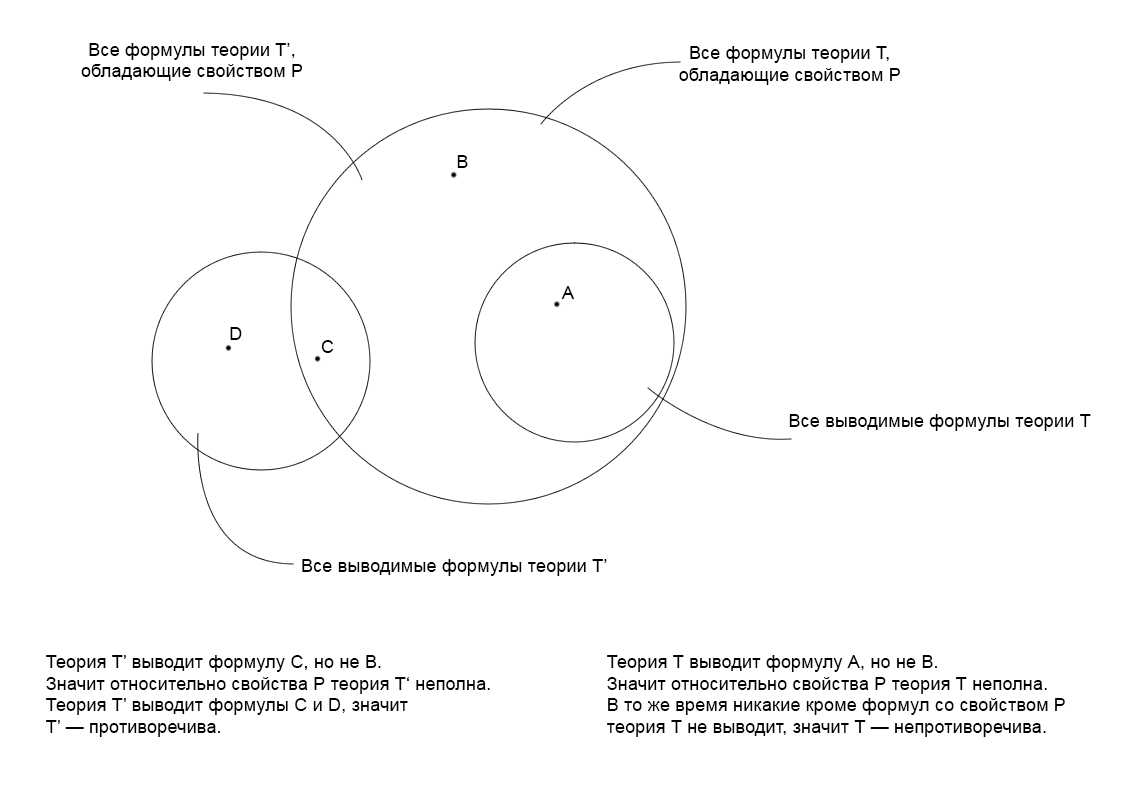
\includegraphics[scale=0.5]{completeness.png}}
		
	\begin{theorem}[\textsection 29, и следствие 1, используется постулат \circled{$8^{\circ}$}]
		Условия теоремы 9 и следствия 1 являются достаточными (так же, как и необходимыми); иначе
		говоря, если $E$ тождественно истинна, то $\vdash E$, и если $E$ и $F$ тождественно равны, то $\vdash E \sim F$.
	\end{theorem}

	\setcounter{theorem}{9}
	
	\begin{theorem}[\textsection 29, Замечание 1]
		Всё доказательство, за исключением последнего шага проходит и в интуиционистской системе.
		Поэтому в последней, для любой пропозициональной формулы $E$, составленной из
		$P_1,\dots,P_m$,
		\begin{itemize}[label={}]
			\setlength\itemsep{0pt}	
			\item \circled{a} $P_1 \vee \neg P_1, \dots, P_m \vee \neg P_m \vdash E$, если $E$ тождественно истинна. 
			\item \circled{b} $P_1 \vee \neg P_1, \dots, P_m \vee \neg P_m \vdash E \vee \neg E$ 
		\end{itemize}
	\end{theorem}
	
	\setcounter{theorem}{9}
	
	\begin{theorem}[\textsection 29, Следствие 2, используется постулат \circled{$8^{\circ}$}]
		Добавление недоказуемой пропозициональной формулы в качестве схемы аксиом к перечню
		постулатов исчисления высказываний нарушает простую непротиворечивость последнего.
	\end{theorem}

	\begin{theorem}[\textsection 29, используется постулат \circled{$8^{\circ}$}]
		Пропозициональная формула $E$, составленная из различных пропозициональных букв $P_1,
		\dots, P_m$, эквивалентна некоторой формуле $F$ (называемой совершенной дизъюнктивной
		нормальной формой формулы $E$), имеющей один из следующих видов. Если $E$ принимает
		значение $t$ для некоторых $m$-ок, составленных из $t$ и $f$ в качестве значений $P_1,
		\dots, P_m$, то $F$ --- дизъюнкция (в некотором порядке) соответствующих элементарных
		конъюнкций. Если $E$ тождественно ложна, то $F$ есть $P_1 \conj \neg P_1$. (Двойственным
		образом, $E$ имеет совершенную конъюнктивную нормальную форму $G$, в которой переставлены
		роли $\vee$ и $\conj$, а также $t$ и $f$; $\vdash E \sim G$) 
	\end{theorem}

	\subsection*{Разрешающая процедура, интерпретация}
	
	В математике известны примеры таких общих вопросов, что на любой частный случай этого вопроса
	может быть дан ответ посредством заранее предписанного единого метода. Точнее, во всяком
	примере такого рода имеется бесконечный класс частных вопросов и связанная с этим классом
	процедура, причём тот и другая описаны заранее таким образом, что если мы выберем любой
	частный вопрос из этого класса, то наша процедура наверное будет применима к этому вопросу и
	даст нам на него определённый ответ ``да'' или ``нет''.
	
	\begin{definition}[\textsection 30]
		Такого рода метод, позволяющий ответить ``да'' или ``нет'' на любой частный случай общего
		вопроса, мы будем называть \textit{разрешающей процедурой}, или \textit{разрешающим
		методом} или \textit{алгоритмом} для этого вопроса. Проблема нахождения такого метода
		называется \textit{проблемой разрешимости}. Эта проблема возникает в современной логике у
		Шрёдера[1895], Лёвенгейма[1915] и Гильберта[1918]. Более точное определение того, что
		представляет собой разрешающий метод, будет в \textsection 60, \textsection 61.
	\end{definition}

	\begin{definition}[\textsection 30]
		Аналогично, может иметься \textit{вычисляющая процедура} или \textit{алгоритм вычисления}
		(а потому и \textit{проблема вычислимости}) в связи с общим вопросом, который требует для
		ответа не ``да'' или ``нет'', а построения некоторого объекта.
	\end{definition}

	\begin{theorem}[\textsection 30, используется постулат \circled{$8^{\circ}$}]
		Алгоритм для определения того, доказуема или нет в исчислении высказываний
		пропозициональная формула $E$, даётся процессом вычисления таблицы для функции от $t$ и
		$f$, представляемой формулой $E$. $E$ доказуема или нет в соответствии с тем, только ли
		$t$ или нет входит в столбец значений.
	\end{theorem}

	Наш метаматематический результат, состоящий в том, что исчисление высказываний допускает
	интерпретацию в арифметике из двух объектов $t$, $f$ является иллюстрацией обычной логической
	интерпретации (см. конец \textsection 28). Мы видим, что наше исчисление высказываний является
	подходящим логическим инструментом,
	\begin{itemize}[label={}]
		\setlength\itemsep{0pt}	
		\item \circled{1} когда конкретные высказывания таковы, что каждое, несомненно, является истинным или ложным или
		\item \circled{2} когда мы хотим, чтобы в рассматриваемой теории имелось допущение, что каждое высказывание истинно или ложно.
	\end{itemize}

	Для интуиционистов ситуация \circled{1} имеет место в математике конечной области предметов, а
	также в рассуждения с высказываниями об объектах бесконечной области, если эти высказывания
	относятся к типу, для которого имеются разрешающие методы (см. замечание 1 \textsection 29).
	Примером ситуации \circled{2} может служить употребление исчисления высказываний в
	классической математике.
\end{document}
